\documentclass[twosided]{report}

% Packages %
\usepackage{fancyhdr}
\usepackage{titling}
\usepackage{graphicx}
\usepackage{xcolor}
\usepackage{listings}
\usepackage{algorithm}
\usepackage{algorithmic}
\usepackage{framed}
\usepackage{enumerate}
\usepackage[hidelinks]{hyperref}
\usepackage{soul}

\hypersetup{linktoc=all}

% Stylings %
\pagestyle{fancy}

% Commands %
\newcommand{\subtitle}[1]{%
  \posttitle{%
    \par\end{center}
    \begin{center}\large#1\end{center}
    \vskip0.5em}%
}

% Colors %
\definecolor{sblgrey}{RGB}{100, 100, 100}
%\definecolor{sblbackground}{RGB}{39, 40, 34}
%\definecolor{sblkeyword}{RGB}{246, 39, 113}
%\definecolor{sbltext}{RGB}{248, 242, 242}
%\definecolor{sblcomment}{RGB}{94, 109, 94}
%\definecolor{sblstring}{RGB}{230, 219, 101} 
\definecolor{sblbackground}{RGB}{241, 240, 236}
\definecolor{sblkeyword}{RGB}{255, 39, 103}
\definecolor{sbltext}{RGB}{7, 13, 13}
\definecolor{sblcomment}{RGB}{94, 109, 94}
\definecolor{sblstring}{RGB}{25, 46, 154}

% Footer/Header %
\fancyhead[LE,RO]{\slshape Chapter \thechapter}
\fancyhead[LO,RE]{\slshape \nouppercase\rightmark}
\fancyfoot[C]{\thepage}

\newcommand{\HRule}{\rule{\linewidth}{0.5mm}}

\lstdefinestyle{fstar}{
	backgroundcolor=\color{sblbackground},
	tabsize=1,
	captionpos=b
  	belowcaptionskip=1\baselineskip,
  	breaklines=true,
  	frame=single,
	frameround=tttt,
	captionpos=b,
  	language=Caml,
	morekeywords={open, module, val, assert},
	showspaces=false,
  	showstringspaces=false,
	showtabs=false,
  	numbers=left,
  	numbersep=5pt,
  	numberstyle=\tiny\ttfamily\color{sblgrey},
	xleftmargin=\parindent,
  	basicstyle=\footnotesize\ttfamily\color{sbltext},
  	keywordstyle=\bfseries\color{sblkeyword},
	otherkeywords={=, :, |},
  	stringstyle=\color{sblstring},
	commentstyle=\color{sblcomment},
	%literate={0}{\textcolor{blue}{0}}
}

\begin{document}

\begin{titlepage}
\begin{center}


\includegraphics[scale=0.4]{images/ITULogo.jpg}\\[1cm]

\textsc{\LARGE IT University of Copenhagen}\\[1.5cm]

\textsc{\Large Bachelor Project}\\[0.5cm]


% Title
\HRule \\[0.4cm]
{\huge \bfseries Verifiable Secure Open Source Alternative to NemID}\\[0.1cm]
\HRule \\[1.5cm]

% Author and supervisor
\begin{minipage}[t]{0.45\textwidth}
\begin{flushleft} \large
\emph{Authors:}
\\[10pt]
Andreas Hallberg \textsc{Kjeldsen}\\
\emph{ahal@itu.dk}
\\[10pt]
Morten Chabert \textsc{Eskesen}\\
\emph{mche@itu.dk}\\
\end{flushleft}
\end{minipage}
\begin{minipage}[t]{0.45\textwidth}
\begin{flushright} \large
\emph{Supervisor:}
\\[10pt]
Dr. Joseph Roland \textsc{KINIRY}\\
\emph{josr@itu.dk}
\\[10pt]
\emph{Co-supervisor:}
\\[10pt]
Hannes \textsc{Mehnert}\\
\emph{hame@itu.dk}
\end{flushright}
\end{minipage}

\vfill

% Bottom of the page
{\large May 22, 2013}

\end{center}
\end{titlepage}


\begin{abstract}
Your abstract goes here...
\end{abstract}

%\renewcommand{\abstractname}{Acknowledgements}
%\begin{abstract}
%Thanks Joe! Thanks Hannes! Rock on!
%\end{abstract}

\begingroup
    \let\clearpage\relax
	\tableofcontents
    \listoffigures
	\lstlistoflistings
\endgroup

\chapter{Introduction}
\emph{Security through obscurity} is a principal within security engineering. It refers to the reliance on secrecy of the design or implementation of a system to provide security. Kerckhoffs's principle also dictates that a cryptographic system where the only private information is the key should be secure.
\begin{quote}
\textit{"There is no security by obscurity"} - Auguste Kerckhoffs \cite{kerckhoffs}
\end{quote}

Based on this, it can be assumed that in the making of a secure system obscurity should not be used for improving the security.
\begin{quote}
\textit{"A system is secure only when it is secure in the light of day, under full public view."} - Dr. Joseph Roland Kiniry \cite{ftspeech}
\end{quote}
\par
In Denmark it is required to use NemID when accessing public websites, online banks and other services requiring a digital signature (DanskeSpil e.g.). NemID claims to be a secure system, they state various reason that would give the impression that they are right \cite{omnemsikkerhed}. But looking at the system from the outside, there is no way of telling if they're right.
\par
Even though there is no public record of the NemID system being completely compromised, there is no way for us outsiders to verify whether or not it could happen. This is due to NemID following the security through obscurity principal. The source code for their key components are not publicly available, the Java applet they are providing has been obfuscated and the API they have made available does not reveal enough to conclude anything.

\section{Objectives}
In this project we set out to create a replacement for NemID that is both verifiable secure and also open source. For the sake of being able to reference this new system throughout the report, we will refer to it as \emph{OpenNemID}.
\par
The goal of this project is to:
\begin{enumerate}
	\item Describe and outline the OpenNemID protocol, including but not limited to registration and login.
	\item Formalize the specification of OpenNemID in F* to the extent possible.
\end{enumerate}

\section{Scope}
This project has had it focus towards specifying a new protocol that could replace NemID. The intent of this project is therefore not to develop a complete system, but to make the specification for a system that could then later be developed based on the specification.

\section{Background}
We're extending the work done by Jacob H{\o}jgaard in his Masters thesis 'Securing Single Sign-On Systems With Executable Models'. Jacobs research has focused on the current implementation of NemID and therefore describes, outlines and models the current system used in Denmark as of May 2013.
\par
NemID is a part of NemLog-in, which is owned by the Danish government through the Agency of Digitalization, henceforth \emph{DIGST}. NemLog-in is a key component in the ambitious digitalization strategy outlined by the DIGST \cite{digst}. The digitalization strategy specifies that all interaction between residents and any public institution should be possible online from 2015. A public login federation\footnote{Login federation refers to the concept of federated identity where a user can link identities stored in different identity management systems. The term \emph{Federation} refers to a union of selfgoverning states, which is very applicable for this term \cite{jacob}.}, NemLog-in, is used for this purpose.
\par
Nets DanID\footnote{Nets DanID A/S is a company within the Nets group, which is owned by the danish national bank and a number of danish banks}, has developed NemID. Their contract runs from august 21st 2008 to august 20th 2015, though the contract can be extended twice, each time by a one year period \cite{nemidcontract}. When the current contract expires it is possible that a new contract mandating a replacement for NemID could be established.
\par
From an academic point of view it would be interesting to see if a replacement for NemID can be made by students within a very limited time frame, that does not rely on hidden and obfuscated code, but on open source and verification tools to prove the system secure.



\chapter{Technical background}
This chapter will clarify the technical concepts that has been used in this report. It will describe the SAML protocol and the Danish specialization OIOSAML. Furthermore it will describe the concept of static analysis and the reasonings behind choice of specification tool. Lastly it will introduce the concept \emph{N-factor authentication} that has been used in the development of this project.

\section{SAML protocol}
The Security Assertion Markup Language or SAML is an XML based language created for the exchanging of authentication and authorization (security tokens) between different systems or domains, in particular between a service provider and an identity provider. The latest version of SAML is 2.0 released in 2005. SAML specifies three roles: \emph{principal}, \emph{identity provider} and \emph{service provider}. Principal refers to an entity that can be authenticated, therefore both the user and the identity provider and service provider are principals. SAML addresses the problem of web browser single-sign on (SSO). SSO means that the user only has to login once pr identity provider pr session. Practically this means that the user only has to be redirected once to the identity provider for authentication once per session. The identity provider creates a session for the user that can be reused for any subsequent authentication request. SAML specifies 5 core elements - \emph{Assertions}, \emph{Protocols}, \emph{Bindings}, \emph{Profiles} and \emph{Metadata}. See appendix A for examples of assertion and SAML messages.
\par
\emph{Assertions} are security tokens containing statements or claims about a principal. These statements in SAML are called attributes and they usually hold information like name, last name, email etc. The principal is referred to as the \emph{subject} in an assertion.
\par
\emph{Protocols} describe the messages that can be exchanged between the service provider and the identity provider when exchanging \emph{assertions}. The protocol used in OpenNemID is called the Authentication Request Protocol. This protocol consists of AuthnRequest message and a response message. The AuthnRequest message has an id that must be unique and the creator of the message is responsible for ensuring it is. The response message has a field \emph{inResponseTo} that specifies the id of the AuthnRequest the response is to.
\par
\emph{Bindings} specifies how the messages are mapped to the underlying HTTP(s) or SOAP protocols. However in this report only HTTP POST and HTTP REDIRECT bindings will be addressed. The POST binding maps the content of messages to hidden XHTML form fields that are named SAMLRequest and SAMLResponse. The content is BASE64 encoded. For the REDIRECT binding the message content is mapped the URL query string with SAMLRequest and SAMLResponse as the identifier. Since the URL query string has limited capacity the message is compressed by the DEFLATE algorithm and after that it is BASE64 encoded and URL encoded.
\par
\emph{Profiles} specifies how the \emph{assertion}, \emph{protocol} and \emph{binding} are used to fulfill a specific requirement or a use case. The Danish specialization of the SAML Web Browser SSO Profile, OIOSAML, will be described in further detail in section 2.1.1.
\par
\emph{Metadata} is the necessary data exchanged between the involved parties in order to know each other. A service provider's metadata contains the certificate for signing messages and a message that the identity provider should use for encrypting assertion. It also contains endpoints which specifies the addresses to which the identity provider should send response messages. More than one endpoint if different bindings are available. The identity provider's metadata also contains signing and encryption certificates and endpoints that specify the addresses for sending requests to the identity provider. Again more endpoints for different bindings. The identity provider will publish the attributes it is able to serve through it's metadata.

\subsection{OIOSAML}

\section{Static analysis}

\section{Selection of specification tool}


\section{N-factor authentication}
\label{sect:nfactauth}



%%%%%%%%%% CHAPTER %%%%%%%%%%
\chapter{Modelling the protocol}
Before formalizing the protocol, it's required to specify and explain some of the words, concepts and meanings used within the protocol. This will be done by using graphical representation of the message flow.

\section{A protocol walkthrough}
A sequence diagram depicting the protocol is useful for introducing the basics of the protocol. The sequence diagrams give a brief overview of the logon protocol, identity provider registration protocol and the user registration protocol. The logon protocol will, later in this chapter, be modeled using a communication diagram, this is done to give a more thorough overview.

\subsection{Logon protocol}
Jacob have depicted the NemID protocol with 12 steps. The sequence diagram shows how the browser must delegate messages from the service provider to the identity provider, while also having to delegate messages from DanId to the identity provider. A single challenge is used to authenticate the user after credentials have been submitted.

\begin{figure}[H]
	\centering
	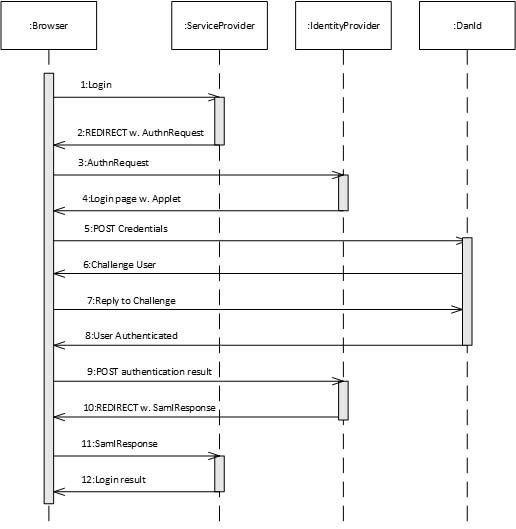
\includegraphics{images/Sequence-login-Jacob.jpg}
	\caption[Sequence diagram of authentication with NemID]{Sequence diagram of authentication with NemID \cite{jacob}}
\end{figure}

In comparison to NemID, the OpenNemID protocol have modified the way messages are sent. The amount of messages the browser must delegate has been limited to few. There is not just one challenge used to authenticate the user, there is N challenges, as described in section \ref{sect:nfactauth}. The amount of steps in the protocol have been reduced to 8.

\begin{figure}[H]
	\centering
	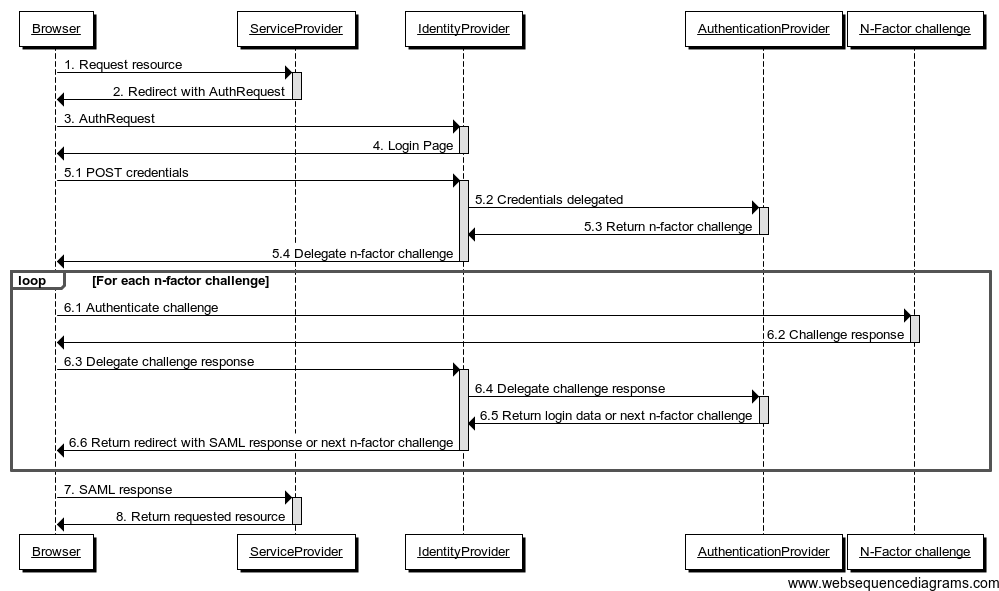
\includegraphics[scale=0.4]{images/Open-NemId-(User-Login).png}
	\caption{Sequence diagram of authentication with OpenNemID}
\end{figure}

\subsection{Identity provider registration protocol}
An identity provider has to register with an authentication provider to establish a trusted relationship and an agreement that the authentication provider will in fact act as a provider for authenticating users. A challenge will be send to the identity provider to confirm that the identity provider is who they claim to be.

\begin{figure}[H]
	\centering
	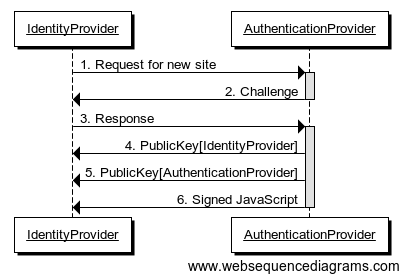
\includegraphics[scale=0.6]{images/Open-NemId-(IdentityProvider-Registration).png}
	\caption{Sequence diagram of identity provider registration with OpenNemID}
\end{figure}

\subsection{User registration protocol}
Before a user is able to authenticate at the authentication provider, they have to register there first. The user has to activate their account using credentials received via mail. Upon activation, a new password must be chosen, optionally a userid can also be chosen. The user must be able to add and revoke N-Factor challenges while also being able to revoke previously granted identity provider permissions.

\begin{figure}[H]
	\centering
	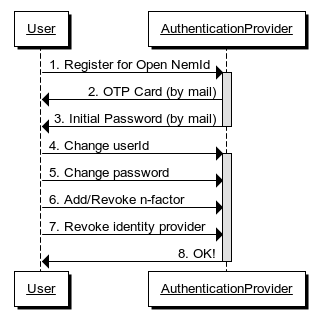
\includegraphics[scale=0.6]{images/Open-NemId-(User-Registration).png}
	\caption{Sequence diagram of user registration with OpenNemID}
\end{figure}

\section{Protocol prerequisites}
It's important to have some requirements as to how the systems should function. The requirements helps define certain properties the involved participants must have or obey to.
It's important to have some requirements as to how the systems should function. The requirements helps define certain properties the involved participants must have or obey to.

\subsection{Shared}
The NemLog-in specification mandates the use of OIOSAML, this will most likely not be excluded, therefore we assume that OpenNemID also has to use it. Further OIOSAML mandates the use of one-way SSL/TLS for all bindings, the mandate does not specify a specific version, though it can be assumed that a minimum version of SSL 3.0 due to the fact that SSL 2.0 is in general considered deprecated. We assume the use of SSL 3.0 or TLS 1.0 in this report.
\par
As mentioned before, SAML uses the browser to transfer messages from one principal to the other. The way to do this is through HTTP REDIRECTs, which could be either a HTTP-GET REDIRECT or a HTTP-POST REDIRECT. The HTTP protocol accepts a Location head in the HTTP RESPONSE which indicates where the browser should redirect to. The location header redirect will act as a HTTP-GET REQUEST which excludes the usage of POST data, thereby limiting the amount of data that can be transferred. To overcome this problem HTTP-POST REDIRECTs are used, these are not a part of the HTTP protocol, but is synthesized by using JavaScript to emulate a regular HTTP-POST REQUEST. Therefore it is required for the users browser to follow redirects and to have JavaScript enabled.
\par
For there to be any actual messages to flow between the service provider and identity provider, it's assumed that they reside in different domains and are different entities.
\par
The identity provider is only to issue assertions to known service providers, this requires that SAML metadata has been changed beforehand. The certificates used for signing and encrypting has to be checked for revocation and validity whenever used.
\\
\par
\textbf{To summarize:}
\begin{enumerate}
	\item OIOSAML mandates the use of SSL(3.0)/TLS(1.0).
	\item The browser must follow redirects.
	\item The browser must have JavaScript enabled.
	\item Service provider and identity provider are different entities residing in different domains.
	\item SAML metadata must have been exchanged between the service provider and identity provider.
	\item Signature check and encryption requires validity/revocation check of the certificate.
\end{enumerate}

\subsection{NemID specifics}
It's required for the OCES certificates used for signing and encrypting to have been issued by DanID.

\subsection{OpenNemID specifics}
For the communication between the authentication provider and the identity provider, a secure tunnel must have been set up. Further the user must have registered at the authentication provider.
\par
We have assume the availability of a web cryptography API in this report. A web cryptography API has not yet been standardized, but a standardization is being worked on, a draft is available \cite{webcrypto}. 

\section{Formalizing protocol messages}
The UML communication diagrams depicting the protocols are made up of two or more participants, henceforth principals, and the messages flowing through the system. The line between two principals indicates a channel where communication can flow, this channel is assumed to be a secure channel, meaning for HTTP messages, the HTTPS protocol would be used. An arrow indicates the direction of the message and the text on top of the arrow is the message being sent. The messages does not conform to any specific formalism, but follows a simple syntax. Messages are, very applicable, named in accordance with their HTTP protocol verb. The messages are to be interpreted the following way:
\begin{enumerate}
	\item[] \textbf{GET} means a HTTP-GET request, the parameter is the resource being requested.
	\item[] \textbf{POST} means a HTTP-POST request, the parameters are the destination for the request followed by the data being submitted.
	\item[] \textbf{REDIRECT} means either a HTTP-REDIRECT or a JavaScript redirect, whichever is used is not important for the purpose of the description. The parameters are the destination for the redirect followed by the parameters to include in the redirect.
	\item[] \textbf{RESPONSE} means a HTTP-RESPONSE messages. The parameters are either the data included in the response or a HTTP status code indicating the type of the response along with a message, this is used for indicating when error happen.
	\item[] \textbf{DELEGATE} means forwarding the data from the previous request, the parameters are the parameters from the previous request that were to be delegated.
	\item[] \textbf{AUTHENTICATE} is to be interpreted as the sequence of actions required to be authenticated at the specified NFactorChallenge. The AUTHENTICATE message is defined this generically on purpose, as the way a user would authenticate for a NFactorChallenge can vary a lot depending on which technology is used (SMS, Facebook, phone call etc.).
\end{enumerate}

\section{Communication model}
To make the changes from NemID to OpenNemID clear, we will first show the communication diagram for NemID, afterwards we will show the communication diagram for OpenNemID. Both diagrams make use of abbreviations, these abbreviations are listed at the top of the diagram along the word or phrase they abbreviate. We have tried to comply with Jacobs data as much as possible, due to the fact that his report conforms to the requirements mandated by Digitaliseringsstyrrelsen.

\subsection{Message processing}
Information regarding the processing of messages have not been included in the diagrams, this is to prevent cluttering of the diagrams. To circumvent this, the processing rules will be described afterwards. The descriptions will be linked to a specific process number, meaning Process 3 would be the handling and response of message 3 in the diagram. Messages that are self-explanatory will not be further described.

\subsection{Communication diagram for NemID}
Description of the message processing for this diagram has been left out of our report, they can however be found in Jacob H{\o}jgaards report \cite{jacob}.

\begin{figure}[H]
	\centering
	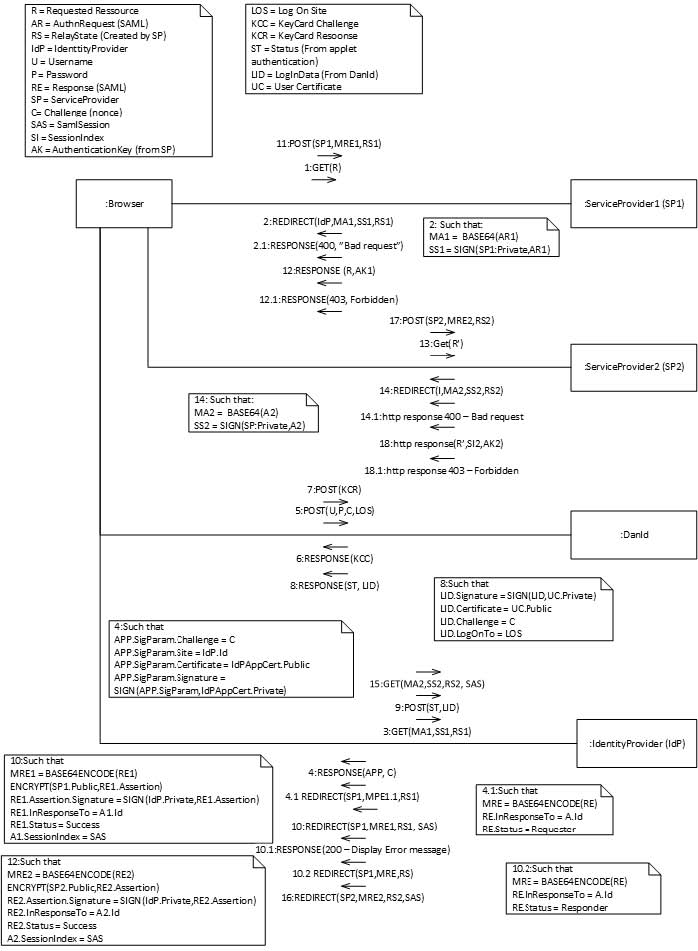
\includegraphics{images/Communication-Jacob.jpg}
	\caption[Communication diagram for the complete NemID protocol]{Communication diagram for the complete NemID protocol \cite{jacob}}
	\label{fig:jacobCommunication}
\end{figure}

\subsection{Communication diagram for OpenNemID}
In this diagram, we have chosen to leave out the additional request to another service provider than the one initially used, this is due to the communication flow being exactly the same as in Jacobs diagram, see Figure \ref{fig:jacobCommunication}, message 13 to 18.
\par
In the communication diagram for OpenNemID, DanID have been replaced by AuthenticationProvider, for the sake of our protocol it is of no greater importance which company handles the authentication.
\par
We have strived to minimize the amount of messages flowing through the system to limit the amount of possible attack points for a potential adversary. We have also eliminated the need for transporting sensitive data, such as the users login data, from the authentication provider to the identity provider, by mandating that the identity provider and the authentication provider exchange information using a secure tunnel without the user being able to interfere.

\begin{figure}[H]
	\centering
	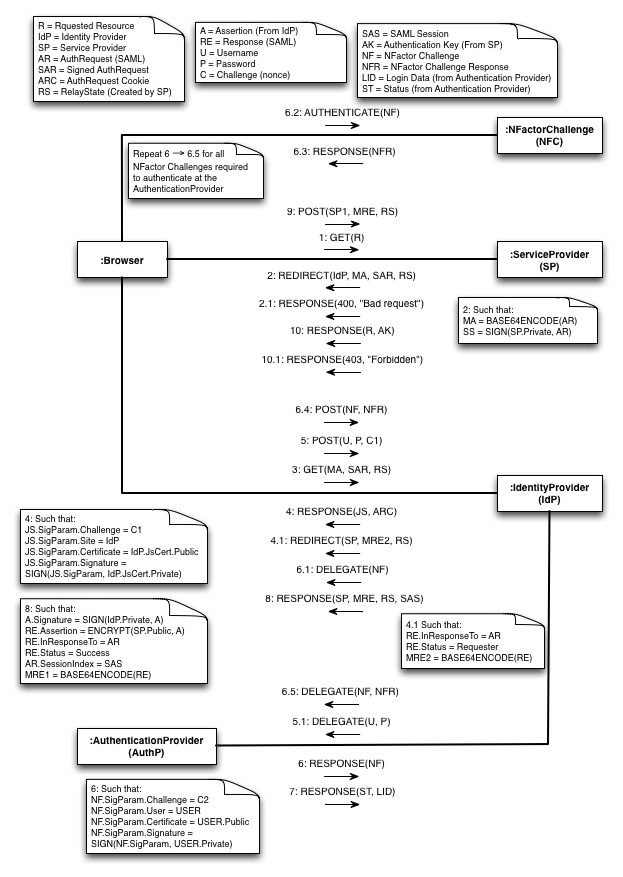
\includegraphics[scale=0.6]{images/Communication.png}
	\caption{Communication diagram for the OpenNemID protocol}
	\label{fig:ourCommunication}
\end{figure}

\subsubsection{Message descriptions}
Process 1 describes the creation of the AuthRequest at the service provider when a resource has been requested. Is the request resource not found a 400 Bad-Request message is returned. The use of url encoding (UrlEnc) and base64 encoding (Base64Enc) is to ensure that the data can be transferred as parameters in the URL.
\par
SAML and OIOSAML has a substantial amount of processing rules that dictates the processing of messages, disobeying these will cause an error. For the sake of communication the descriptions have been kept to a minimum, not listening all scenarios that would cause an error.

\begin{algorithm}[H]
	\caption{Process 1}
	\begin{algorithmic}
	\REQUIRE{GET is well-formed \AND IdP.Public \AND SP.Private}
	\IF{R exists}
		\STATE AR $\leftarrow$ CreateAuthRequest()
		\STATE SAR $\leftarrow$ SIGN(AR, SP.Private)
		\STATE MA $\leftarrow$ UrlEnc(Base64Enc(DeflateCompress(AR)))
		\STATE RS $\leftarrow$ UrlEnc(Base64Enc(R))
		\RETURN REDIRECT(IdP, MA, SAR, RS)
	\ELSE
		\RETURN RESPONSE(400, Bad−Request)
	\ENDIF
	\end{algorithmic}
\end{algorithm}

Process 3 describes the handling of a \emph{AuthRequest} at the identity provider. The request will be handled in one of two ways depending on whether the AuthRequest could be verified. In the case of verification failing, a SAML response will be returned indicating an error. Otherwise a page for requesting the users credentials is returned. The page returned will also contains the signed JavaScript for handling the OpenNemID specific actions. The JavaScript is signed using a certificate, \emph{IdPJsCert}, this certificate has to have been issued by the authentication provider.
\par
A challenge (nonce) is generated, this is to prevent an attack where an adversary would submit an identical request to one that has already been submitted, also known as a \emph{replay attack}. If the challenge wasn't introduced the second identical request would also be accepted.
\par
A cookie is created containing the AuthRequest, signed AuthRequest along with the relay state. This is done to free the identity provider from having to store the data, thereby granting more statelessness.
\begin{algorithm}[H]
	\caption{Process 3}
	\begin{algorithmic}
		\REQUIRE{GET is well-formed \AND IdP.Private \AND SP.Public \AND IdPJsCert.Public \AND IdP has JavaScript from AuthP}
		\STATE AR $\leftarrow$ DeflateDecompress(Base64Dec(UrlDec(MA)))
		\IF{VERIFY(AR, SAR, SP.Public)}
			\STATE C1 $\leftarrow$ GenChallenge()
			\STATE JS $\leftarrow$ GetStoredJavaScript()
			\STATE JS.SigParams.Challenge $\leftarrow$ C1
			\STATE JS.SigParams.Certificate $\leftarrow$ IdPJsCert.Public
			\STATE JS.SigParams.Signature $\leftarrow$ SIGN(JS.SigParams, IdPJsCert.Private)
			\STATE ARC $\leftarrow$ CreateCookie(MA, SAR, RS)
			\RETURN RESPONSE(JS, ARC)
		\ELSE
			\STATE RE $\leftarrow$ CreateResponse()
			\STATE RE.InResponseTo $\leftarrow$ AR
			\STATE RE.Status $\leftarrow$ ”Requester”
			\STATE MRE $\leftarrow$ Base64Enc(RE)
			\RETURN REDIRECT(SP, MRE, RS)
		\ENDIF
	\end{algorithmic}
\end{algorithm}

As specified in the formalization, it's required for the browser to allow JavaScript. The username, \emph{U} and password, \emph{P} for the user is not stored and fetched directly, but will be input by the user manually, though for the description of process 4 it will be assumed that they are both ready right away. Before the user is prompted for username and password, the JavaScript is verified. The challenge is submitted together with the username and password. Hashing of the username and password has been omitted as it holds no functional enhancement towards the protocol.
\begin{algorithm}[H]
	\caption{Process 4}
	\begin{algorithmic}
		\REQUIRE{U \AND P \AND Browser allows JavaScript}
		\STATE SigParams $\leftarrow$ Js.SigParams
		\IF{VERIFY(SigParams, SigParams.Signature, SigParams.Certificate)}
			\STATE C1 $\leftarrow$ SigParams.Challenge
			\RETURN POST(U, P, C1)
		\ELSE
			\PRINT ERROR
		\ENDIF
	\end{algorithmic}
\end{algorithm}

In process 5 the identity provider confirms that the challenge received matches a previously issued challenge, and that is has not already been used. A SAML response indicating an error is returned if the challenge is not accepted, otherwise the username and password will be delegated to the authentication provider.
\begin{algorithm}[H]
	\caption{Process 5}
	\begin{algorithmic}
		\REQUIRE{POST is well formed}
		\IF{C1 matches challenge issued by IdP \AND C1 is valid}
			\STATE \textbf{Delegate} U \AND P \TO AuthP
		\ELSE
			\RETURN RESPONSE(ERROR)
		\ENDIF
	\end{algorithmic}
\end{algorithm}

Process 5.1 describes how the username and password submitted is used to identify a user at the authentication provider. If a user is found and is valid, a challenge will be generated and the next N-Factor challenge for the user will be fetched. The N-Factor challenge is signed and then returned. Were no valid user found based on the supplied username and password, a SAML response message indicating an error will be returned.
\begin{algorithm}[H]
	\caption{Process 5.1}
	\begin{algorithmic}
		\STATE USER $\leftarrow$ GetUser(U, P)
		\IF{USER is valid}
			\STATE C2 $\leftarrow$ GenChallenge()
			\STATE NF $\leftarrow$ GetNextNFactorChallenge(USER)
			\STATE NF.SigParam.User $\leftarrow$ USER
			\STATE NF.SigParam.Challenge $\leftarrow$ C2
			\STATE NF.SigParam.Certificate $\leftarrow$ USER.Public
			\STATE NF.SigParam.Signature $\leftarrow$ SIGN(NF.SigParam, USER.Private)
			\RETURN RESPONSE(NF)
		\ELSE
			\RETURN RESPONSE(ERROR)
		\ENDIF
	\end{algorithmic}
\end{algorithm}

Process 6 show how the identity provider has to delegate messages from the browser to the authentication provider and vice versa. In this case the N-Factor challenge is to be delegated. If the authentication provider returned an error or the identity provider cannot verify the N-Factor challenge received, a SAML response message indicating an error will be returned to the browser. If the N-Factor challenge is verified, it is then delegated to the browser.
\begin{algorithm}[H]
	\caption{Process 6}
	\begin{algorithmic}
		\STATE SigParams $\leftarrow$ NF.SigParams
		\IF{VERIFY(SigParams, SigParams.Signature, SigParams.Certificate)}
			%\STATE RELATE(SigParams.User, SigParams.Challenge)
			\STATE \textbf{Delegate} NF \TO Browser
		\ELSE
			\STATE \textbf{Delegate} ERROR \TO Browser
		\ENDIF
	\end{algorithmic}
\end{algorithm}

The browser also verifies that the N-Factor challenge is valid in process 6.1. An attempt to authenticate the N-Factor challenge is then performed. Due to the challenges genericity, the authentication process will not be further described.
\begin{algorithm}[H]
	\caption{Process 6.1}
	\begin{algorithmic}
		\STATE SigParams $\leftarrow$ NF.SigParams
		\IF{VERIFY(SigParams, SigParams.Signature, SigParams.Certificate)}
			\STATE AUTHENTICATE(NF)
		\ELSE
			\PRINT ERROR
		\ENDIF
	\end{algorithmic}
\end{algorithm}

In process 6.2, the genericity of the N-Factor challenges once more results in a minimal description. The way the authentication attempts will be handled depends on the N-Factor challenge, therefore to simplify the description, it is assumed that a result conforming to a specific template is returned.
\begin{algorithm}[H]
	\caption{Process 6.2}
	\begin{algorithmic}
		\STATE NFR $\leftarrow$ NFactorResult(NF)
		\RETURN RESPONSE(NFR)
	\end{algorithmic}
\end{algorithm}

Process 6.5 describes the handling of a N-Factor challenge result. First off, the N-Factor challenge is verified to make sure that it has not been altered. Then it is checked whether or not the N-Factor challenge result is acceptable for the N-Factor challenge. In the case of acceptance the user is fetched. If the user has not yet completed all N-Factor challenges required to authenticate at the authentication provider, then the next challenge is fetched, signed and returned to the user. Process 6 to 6.5 is then repeated until no more N-Factor challenges are required, in which case login data for the user is created and returned to the identity provider. In case of the N-Factor challenge not passing verification or the N-Factor challenge result is not accepted a SAML message indicating an error is returned.
\begin{algorithm}[H]
	\caption{Process 6.5}
	\begin{algorithmic}
		\REQUIRE{User identifiable by (NF.SigParams.USER, NF.SigParams.Certificate)}
		\STATE SigParams $\leftarrow$ NF.SigParams
		\IF{VERIFY(SigParams, SigParams.Signature, SigParams.Certificate)}
			\IF{NFR is acceptable result of NF}
				\STATE USER $\leftarrow$ GetUser(SigParams.USER, SigParams.Certificate)
				\STATE C2 $\leftarrow$ GenChallenge()
				\IF{USER.HasNextChallenge}
					\STATE NF $\leftarrow$ GetNextNFactorChallenge(USER)
					\STATE NF.SigParams.User $\leftarrow$ USER
					\STATE NF.SigParams.Challenge $\leftarrow$ C2
					\STATE NF.SigParams.Certificate $\leftarrow$ USER.Public
					\STATE NF.SigParams.Signature $\leftarrow$ SIGN(NF.SigParams, USER.Private)
					\RETURN RESPONSE(NF)
				\ELSE
					\STATE LID $\leftarrow$ CreateLogInData(USER)
					\STATE ST $\leftarrow$ "OK"
					\RETURN RESPONSE(ST, LID)
				\ENDIF
			\ELSE
				\RETURN RESPONSE(ERROR)
			\ENDIF
		\ELSE
			\RETURN RESPONSE(ERROR)
		\ENDIF	
	\end{algorithmic}
\end{algorithm}

In process 7 it is described how the identity provider handles when a user has been authenticated at the authentication provider. If the returned status does not equal an acceptance criteria, the status is returned to the browser to indicate an error, the status would further describe the error. When the status is accepted the cookie created in process 3 is fetched and the contents on the cookie are extracted.
\par
The initial AuthRequest extracted from the cookie is verified. Verification failure results in the user being redirected to the service provider with information indicating that the AuthRequest could not be granted.
\par
When verification succeeds, an assertion is build based on the login data received from the authentication provider. The assertion is then encrypted using the service providers public key. A SAML response is created, the assertion is appended to it along with the AuthRequest. The browser is then redirected to the service provider.
\begin{algorithm}[H]
	\title{negermand}
	\caption{Process 7}
	\begin{algorithmic}
		\REQUIRE{SP.Public \AND LID is well-formed \AND ARC cookie present}
		\IF{ST = "OK"}
			\STATE MA $\leftarrow$ ARC.AR
			\STATE SAR $\leftarrow$ ARC.SAR
			\STATE RS $\leftarrow$ ARC.RS
			\STATE AR $\leftarrow$ DeflateDecompress(Base64Dec(UrlDec(MA)))
			\IF{VERIFY(AR, SAR, SP.Public)}
				\STATE A $\leftarrow$ BuildAssertion(LID.Certificate)
				\STATE SI $\leftarrow$ GenerateSessionIndex()
				\STATE A.InResponseTo $\leftarrow$ AR
				\STATE A.Issuer $\leftarrow$ IdP
				\STATE A.Audience $\leftarrow$ SP
				\STATE A.SessionIndex $\leftarrow$ SI
				\STATE A.Signature $\leftarrow$ SIGN(A, IdP.Private)
				\STATE EA $\leftarrow$ ENCRYPT(A, SP.Public)
				\STATE RE $\leftarrow$ CreateResponse()
				\STATE RE.Assertion $\leftarrow$ EA
				\STATE RE.InResponseTo $\leftarrow$ AR
				\STATE RE.Status $\leftarrow$ "Success"
				\STATE MRE $\leftarrow$ DeflateCompress(Base64Enc(UrlEnc(RE)))
				\STATE SAS $\leftarrow$ CreateSAMLSession(SI, SP, LID.CertificateSubject)
				\RETURN REDIRECT(SP, MRE, RS, SAS)
			\ELSE
				\STATE RE $\leftarrow$ CreateResponse()
				\STATE RE.InResponseTo $\leftarrow$ AR
				\STATE RE.Status $\leftarrow$ "Requester"
				\STATE MRE $\leftarrow$ DeflateCompress(Base64Enc(UrlEnc(RE)))
				\RETURN REDIRECT(SP, MRE, RS)
			\ENDIF	
		\ELSE
			\RETURN RESPONSE(ST)
		\ENDIF
	\end{algorithmic}
\end{algorithm}

Process 9 describes the last step in the diagram. The SAML response is received at the service provider. The assertion is decrypted and verified. If the verification fails an error message is returned to the browser. If the verification succeeds, an AuthKey is generated. If the user supplies the AuthKey in subsequent requests to the service provider, the service provider will know that the user already allowed to view its resources thereby eliminating the need to authenticate again until the AuthKey expires. The initial requested resource is retrieved and returned to the browser together with the AuthKey.
\begin{algorithm}[H]
	\caption{Process 9}
	\begin{algorithmic}
		\REQUIRE{POST is well.formed \AND SP.Private \AND IdP.Public}
		\STATE RE $\leftarrow$ UrlDec(Base64Dec(DeflateDecompress(MRE)))
		\STATE A $\leftarrow$ DECRYPT(RE.Assertion, SP.Private)
		\IF{VERIFY(A, A.Signature, IdP.Public)}
			\STATE AK $\leftarrow$ GenAuthKey()
			\STATE R $\leftarrow$ Base64Dec(UrlDec(RS))
			\STATE RES $\leftarrow$ GetResource(R)
			\RETURN RESPONSE(RES, AK)
		\ELSE
			\RETURN RESPONSE(403, Forbidden)
		\ENDIF
	\end{algorithmic}
\end{algorithm}

This concludes the formalizing of the OpenNemID protocol and processing, the subsequent chapter will show how to transform this model into an executable modal using F*.

\chapter{Modelling with F*}
This chapter will introduce the language F* that can be used to model a security protocol. Despite being a formal specification language F* is also executable. F* is described as a \emph{A Verifying Compiler for Distributed Programming}. This chapter will describe how we have used F* to build a formal specification of OpenNemID.

\section{Introducing F*}
F* is a research language from Microsoft Research. F* primarily subsumes two research languages from Microsoft Research, F7\footnote{http://research.microsoft.com/en-us/projects/f7/} and Fine\footnote{http://research.microsoft.com/en-us/projects/fine/}. F* is at this time considered to be an $\alpha$-release.The purpose of designing F* is to enable the construction and communication of proofs of program properties and of properties of a program's environment in a verifiable secure way. F* is a dialect of ML and compiles to .NET bytecode in type-preserving style. This means that it can inter op with other .NET languages and the types defined in F* can be used by other .NET languages without loosing type information. Furthermore there also exists a fully abstract compiler from F* to JavaScript. This makes it possible to deploy F* programs on web pages as JavaScript meanwhile there is a formal guarantee that the program still behaves just as they would according to F* semantics. The compiling and type-checking of F* code utilizes the Z3\footnote{http://z3.codeplex.com/} SMT solver for proving assumptions made with refinement types. F* has been formalized and verified using Coq\footnote{Coq is an interactive theorem prover written in OCaml}.

\section{Syntax and semantics}
F* inherits syntax and semantics from ML. F* is a functional language which means that it has features like immutability by default, polymorphic types and type inference. In Listing 4.1 we have shown the classic Hello World example in F*. This is the simplest way this example could have been written. This example shows how to specify a main method by defining a function \_ (underscore) at the end of a module. This will instruct the compiler to make an .exe file instead of a dll.

\begin{lstlisting}[style=fstar, caption={Hello World example in F*}]
	module HelloWorld
	
	let _ = print "Hello world!"
\end{lstlisting}

The example in listing 4.2 shows how to explicitly specify types with the \emph{colon} operator and the \emph{val} declaration for defining function signatures. This example defines the function multiply that takes two ints as parameters and returns an int. After that it defines the corresponding \emph{let} binding which defines multiplies the 2 arguments. It is important to note that not defining the corresponding let binding will not cause the compilation to fail but give the following warning: \emph{Warning: Admitting value declaration Multiplication.multiply as an axiom without a corresponding definition}. So the value declaration was valid but there is no concrete implementation supporting this claim.

\begin{lstlisting}[style=fstar, caption={Multiplication example in F*}]
	module Multiplication

	val multiply: x:int -> y: int -> int
	
	let multiply x y = x * y
	
	let mul = multiply 3 4
\end{lstlisting}

\section{Refinement types}
F* has derived the feature refinement types from the Microsoft Research projects, F7 and Fine. Refinement types are used to make type safe refinements of existing types. Thus it is possible to restrict or refine values more than their original type. Listing 4.3 shows an example with the refinement \emph{nat} of int that states that \emph{nat} will always be zero of larger, i.e. a natural number. The example also shows an attempt to assign -1 to a type of nat which will fail type checking.
\begin{lstlisting}[style=fstar, caption={Simple refinement types in F*}]
	(*Declare a type nat of natural numbers*)	
	type nat = i:int{0 <= i}
	
	let x:nat = 1
	let y:nat = 0
	let z:nat = 1 - 2 (*Will fail type check*)
\end{lstlisting}

Refinement types have the form $x:t\{t'\}$ as shown above. So a refinement type is created by taking an existing type and decorate it with an expression in curly brackets. In the example above the refinement type is a simple boolean expression but refinements are not limited to boolean expression. This is extended in F* by its kind-system. Kinds can be seen as an abstraction over types - types can either \emph{have} or be \emph{of} a kind. The *-kind indicates 'regular types' in F*. This covers all the possible types to create in a regular type system for a programming language like Java. Refinement types are of the E-kind and not of the *-kind. The E(rasable)-kinds have no significance at runtime. They only have an effect at the compiling time during type checking.

\section{Formalizing OpenNemID by using Jacob's work - THIS IS A BAD TITLE!}
Since we are extending Jacob's work with the authentication part of the protocol we used his code as a reference for implementing the rest of the OpenNemID protocol. In listing 4.4 we show Jacob's implementation of the Identity Provider. He has implemented a recursive function \emph{identityprovider} declared with the \emph{val} binding just above it. The function declared takes 2 arguments and returns \emph{unit}.\\
\textbf{The arguments}
\begin{enumerate}
\item a principal for identifying the identity provider
\item a principal for identifying the client.
\end{enumerate}
\emph{Unit} means the same as void in Java.

\begin{lstlisting}[style=fstar, caption={NemID identity provider implementation \cite{jacob}}]
	module Identityprovider

	open SamlProtocol
	open Crypto

	let handleUserAuthenticated me user client authnrequest =
	  match authnrequest with 
  	| MkAuthnRequest(reqid,issueinst,dest,sp,msg,sigSP) ->
   	   let pubksp = CertStore.GetPublicKey sp in
      
  	    if (VerifySignature sp pubksp msg sigSP) then
  	      (assert (Log sp msg);
 	       let assertion = IssueAssertion me user sp reqid in
 	       let myprivk = CertStore.GetPrivateKey me in
 	       assume(Log me assertion);
  	      let sigAs = Sign me myprivk assertion in
	        let signAssertion = AddSignatureToAssertion assertion sigAs in
	        let encryptedAssertion = EncryptAssertion sp pubksp 
signAssertion in
  	      let resp = AuthResponseMessage me sp encryptedAssertion in
	        SendSaml client resp) (*10*)
	      else
	        SendSaml client (Failed Requester)(*10.2*)

	val identityprovider: me:prin -> client:prin -> unit

	let rec identityprovider me client =
		let req = ReceiveSaml client in (*3 & 11*)
		match req with
		| AuthnRequestMessage (issuer, destination, message, sigSP) ->
 	   let pubkissuer = CertStore.GetPublicKey issuer in
	    if (VerifySignature issuer pubkissuer message sigSP) then
	      (assert (Log issuer message);
 	     let challenge = GenerateNonce me in
	      let resp = UserCredRequest challenge in
	      SendSaml client resp; (*4*)
	      identityprovider me client (*Start over*))
	    else
	      SendSaml client (Failed Requester);(*4.1*)
	      identityprovider me client (*Start over*)

	  | UserAuthenticated (status, logindata, authnrequest) ->
	    match logindata with 
	    | MkLoginData (user,sig,cert,challenge,site,data) ->
	      if (status = "OK") && (VerifySignature user cert data sig) then
	        (assert (Log user data);
	          handleUserAuthenticated me user client authnrequest;
	          identityprovider me client (*Start over*)
 	       )
	      else
	        SendSaml client (DisplayError 400);(*10.1*)
	        identityprovider me client (*Start over*)
 	 | _ -> SendSaml client (DisplayError 400);(*10.1*)
  	      identityprovider me client (*Start over*)
\end{lstlisting}

The recursive function \emph{identityprovider} starts by receiving a SAML message from the client. It then matches the request with a \emph{SamlMessage.AuthnRequestMessage} or\emph{SamlMessage.UserAuthenticated} type. When matched with an AuthnRequest message it verifies the Service Provider's signature of the message by the function \emph{VerifySignature} which is shown in listing 4.5. The function takes a principal, the principals public key, a message and a signature. It returns a boolean indicating if the check passed. The return type however has a refinement type that relates the message to the principal if the verification passes. $==>$ should be as implication therefore stating that the predicate is valid. If the verification of the Service Provider's signature of the AuthnRequestMessage passes it creates a nonce to be related to this user when the user has authenticated himself/herself by NemID and sends the response to the user. When the user has authenticated through NemID the function \emph{handleUserAuthenticated} is called. The function's purpose is to issue a signed assertion and sending the AuthResponseMessage to the user. The signature for signing messages takes 4 arguments - the principal, the signer, the private key of the principal and the message to be signed. The message is annotated with a refinement type \emph{\{Log p msg\}}. This refinement type is an E-kinded type that takes a principal and a string as constructor elements. The val declaration for a method Sign in listing 4.5 requires the predicate \{Log p msg\} to be true before it can typecheck. This means that the message to sign is related to the principal signing the message. Securing this is done by calling \emph{assume\{Log me assertion\}} before signing the message. The predicate is by virtue of this "verified". After this the assertion is encrypted by using the Service Provider's public key and sent within an AuthResponseMessage to the user.

\begin{lstlisting}[style=fstar, caption={Cryptographic elements}]
	type pubkey :: prin => *
	type privkey :: prin => *

	type Log :: prin => string => E
	
	val Sign: p:prin
		-> privkey p
		-> msg:string{Log p msg}
		-> dsig

	val VerifySignature: p:prin
		-> pubkey p 	
		-> msg:string
		-> dsig
		-> b:bool{b=true ==> Log p msg}
\end{lstlisting}

In listing 4.5 we show the declaration of the types for private key (\emph{privkey}) and public key (\emph{pubkey}). These types are declared by using the F* syntax for constructing dependent types (the double colon). This means that a type \emph{pubkey} will have a constructor that takes a \emph{prin} (principal) and returns a type of *-kind. This is still abstract and the type has no actual constructor.

\section{OpenNemID specified in F*}
The code in this section represents the state of the project now. This is in no way a complete implementation of the protocol. Implementation was carried out in an incremental manner. First the focus was on understanding Jacob's work and expanding that with the authentication part (Authentication Provider) of the protocol, which before was done by NemID, and then adding the functionality of creating login, establishing connection between Identity Provider and the Authentication Provider and so on. All source code that has been produced in this project can be found on the source code sharing community Github\footnote{https://github.com/kiniry-supervision/OpenNemID}.
\\The F* code for the protocol is organized in 10 modules:
\begin{enumerate}
	\item The TypeFunc module
	\item The SamlProtocol module
	\item The Crypto module
	\item The CertStore module
	\item The Messaging module
	\item The Service Provider module
	\item The Identity Provider module
	\item The Database module
	\item The Authentication Provider module
	\item The Browser module
\end{enumerate}
The modeling follows the principles for cryptographic protocol modeling outlined by Dolev \& Yao\footnote{Cryptographic primitives are assumed perfect and cyphers cannot be decrypted without the the proper decryption key}. In the following we will explain the important principles for each module and the relation to the algorithms outlined in chapter 3.
\subsection{Specification of the type functionality module}

\begin{lstlisting}[style=fstar, caption={TypeFunc module}]
	module TypeFunc

	type Authentication =
 	 | Facebook: id:int -> Authentication
 	 | SMS: generated:int -> Authentication
	 | Google: id:int -> Authentication
	 | OpenId: id:int -> Authentication
\end{lstlisting}

The \emph{TypeFunc} module provides the type authentication which is used for the different kinds of n factor authentication. Note that currently there is only an id associate with each type of authentication for simplicity. This needs to be modified so that each type is more explicit and holds the correct information for authentication.
\subsection{Specification of the SAML Protocol}

\begin{lstlisting}[style=fstar, caption={Specification of the SAML Protocol elements}]
	module SamlProtocol
	
	open Crypto
	open TypeFunc

	type assertiontoken = string (*Add refinements*)
	type signedtoken = string (*Add refinements*)
	type id = string
	type endpoint = string
	type uri = string


	type AuthnRequest = 
	  | MkAuthnRequest: IssueInstant:string ->
			    Destination:endpoint -> Issuer:prin ->
			    message:string -> sig:dsig ->
			    AuthnRequest

	type LoginData = 
	  | MkLoginData:  user:prin -> signature:dsig ->
			  cert:pubkey user -> challenge:nonce ->
			  site:string -> data:string ->
			  LoginData

	type LoginInfo =
	  | UserLogin:  userid:string -> password:string ->
			LoginInfo

	type AuthInfo =
	  | UserAuth:   userid:string -> authmethod:Authentication ->
			authresponse:Authentication -> AuthInfo

	type Assertion =
	  | SignedAssertion: assertiontoken -> dsig -> Assertion
	  | EncryptedAssertion: cypher -> Assertion

	type SamlStatus =
	  | Success: SamlStatus
	  | Requester: SamlStatus
	  | Responder: SamlStatus

	type LoginError =
	  | AuthError: LoginError
	  | CredentialError: LoginError

	type SamlMessage =
	  | SPLogin: uri -> SamlMessage
	  | Login: loginInfo:LoginInfo -> challenge:nonce -> SamlMessage
	  | LoginResponse: string -> SamlMessage
	  | AuthnRequestMessage: issuer:prin ->  destination:endpoint -> message:string -> dsig -> SamlMessage
	  | LoginRequestMessage: issuer:prin ->  destination:endpoint -> loginInfo:LoginInfo -> SamlMessage 
	  | NfactAuthRequest: issuer:prin -> destination:endpoint -> authInfo:AuthInfo -> challenge:nonce -> dsig -> SamlMessage
	  | AuthResponseMessage: issuer:prin -> destination:endpoint -> Assertion -> SamlMessage
	  | LoginResponseMessage: issuer:prin -> destination:endpoint -> auth:Authentication -> challenge:nonce -> dsig -> SamlMessage
	  | UserAuthenticated: status:string -> logindata:LoginData -> authnReq:AuthnRequest -> SamlMessage
	  | UserCredRequest: javascript:string -> challenge:nonce -> dsig -> SamlMessage
	  | UserAuthRequest: authmethod:Authentication -> challenge:nonce -> dsig -> SamlMessage
	  | UserAuthResponse: authInfo:AuthInfo -> challenge:nonce -> dsig -> SamlMessage
	  | LoginSuccess: status:string -> issuer:prin -> destination:endpoint -> SamlMessage
	  | Failed: SamlStatus -> SamlMessage
	  | LoginFailure: LoginError -> SamlMessage
	  | DisplayError: int -> SamlMessage


	val SendSaml: prin -> SamlMessage -> unit
	val ReceiveSaml: prin -> SamlMessage 

	val CreateAuthnRequestMessage: issuer:prin -> destination:prin -> string
	val IssueAssertion: issuer:prin -> subject:prin -> audience:prin -> inresto:AuthnRequest -> assertiontoken
	val AddSignatureToAssertion: assertiontoken -> dsig -> signedtoken
	val EncryptAssertion: receiver:prin -> pubkey receiver -> signedtoken -> Assertion
	val DecryptAssertion: receiver:prin -> privkey receiver -> Assertion -> (signedtoken * dsig)
\end{lstlisting}

The \emph{SamlProtocol} module is taken directly from Jacob's code and only modified to support more and different \emph{SamlMessage} that are needed in our specification of OpenNemID. This module's purpose is the specification of messages and to provice functions for sending and receiving messages. Note that the functions for sending and receiving messages have no runtime implementation. They are only specified by the \emph{val} declaration. The SAML Protocol is used for the communication between the principals in the OpenNemID protocol in a login session. The intention with these functions is that they will handle the mapping of protocol elements to the network.
\subsection{Specification of cryptographic elements}

\begin{lstlisting}[style=fstar, caption={Specification of cryptographic elements}]
	module Crypto
	
	open Protocol
	open TypeFunc

	type prin = string
	type pubkey :: prin => *
	type privkey :: prin => *
	type dsig
	type nonce = string
	type cypher

	(*Verification*)
	type Log :: prin => string => E

	type LogAuth :: prin => Authentication => E

	val Keygen: p:prin
		  -> (pubkey p * privkey p)

	val Sign: p:prin
		-> privkey p
		-> msg:string{Log p msg}
		-> dsig

	val SignAuth: p:prin
		-> privkey p
		-> msg:Authentication{LogAuth p msg}
		-> dsig

	val VerifySignature: p:prin
		-> pubkey p 
		-> msg:string
		-> dsig
		-> b:bool{b=true ==> Log p msg}

	val VerifySignatureAuth: p:prin
		-> pubkey p 
		-> msg:Authentication
		-> dsig
		-> b:bool{b=true ==> LogAuth p msg}

	val Encrypt: p:prin
		-> pubkey p
		-> string
		-> cypher

	val Decrypt: p:prin
		-> privkey p
		-> cypher
		-> string

	val GenerateNonce: prin -> nonce (*Add refinement to ensure unqueness*)
\end{lstlisting}

The \emph{crypto} module is taken directly from Jacob's code and only modified to support signing and verification of the authentication type. The purpose of the \emph{crypto} is providing the cryptographic functions to sign and verify both messages and the authentication type also the encryption and decryption of messages. The \emph{crypto} module utilizes the refinement type to ensure that signed messages and authentications have typed dependency to the signing principal. It does not have a concrete implementation as of now.
\subsection{Specification of certificate store module}

\begin{lstlisting}[style=fstar, caption={Abstract certificate store}]
	module CertStore
	
	open Crypto

	val GetPublicKey: p:prin -> pubkey p
	val GetJSPublicKey: p:prin -> pubkey p
	(*Prin needs to be updated to include credentials*)
	val GetPrivateKey: p:prin -> privkey p 
	val GetJSPrivateKey: p:prin -> privkey p
\end{lstlisting}

The \emph{CertStore} module is taken from Jacob's code and expanded with functionality to support JavaScript public and private keys. This module provides four abstract functions for retrieving certificates from a certificate store. The functions use the value dependent syntax for relating a principal to the certificate keys. As Jacob has written in a comment the principal could be updated to include credentials  because this is a quite naive implementation. It is quite naive because all you need to obtain the private key of a principal is the name of the principal.
\subsection{Specification of the messaging protocol}

\begin{lstlisting}[style=fstar, caption={Specification of the Messaging protocol}]
	module Messaging
	
	open Crypto
	open TypeFunc

	type Status =
		| Successful: Status
		| Unsuccessful: Status

	type Message =
		| NewSiteRequest: idp:prin -> Message
		| ChallengeResponse: challenge:nonce -> Message
		| IdpChalResponse: challenge:nonce -> Message
		| AcceptedIdp: idp:prin -> pubkey:pubkey idp -> authp:prin -> authpubkey:pubkey authp -> signedjavascript:string -> Message
		| RequestForLogin: userid:string -> password:string -> email:string -> Message
		| ReqLoginResponse: challenge:nonce -> Message
		| CreateLogin: generatedpassword:string -> challenge:nonce -> Message
		| ChangeUserId: userid:string -> newUserId:string -> password:string -> Message
		| ChangePassword: userid:string -> password:string -> newPassword:string -> Message
		| UserRevokeIdp: userid:string -> password:string -> idp:string -> Message
		| AddNfactor: userid:string -> password:string -> nfact:Authentication -> Message
		| RemoveNfactor: userid:string -> password:string -> nfact:Authentication -> Message
		| StatusMessage: Status -> Message


	val SendMessage: prin -> Message -> unit
	val ReceiveMessage: prin -> Message
\end{lstlisting}
%\end{shaded}
The \emph{Messaging} module is responsible for 2 things - the specification of messages and providing functions for sending and receiving these messages. As the \emph{SamlProtocol} module the functions for sending and receiving are specified only by the \emph{val} declaration and has no concrete runtime implementation. This module is used to model the communication between Identity Provider / user and the Authentication Provider when wanting to establish a secure connection and creating and/or changing an user's login.
\subsection{Specification of the Service Provider}

\begin{lstlisting}[style=fstar, caption={Specification of service provider}]
	module Serviceprovider
	
	open SamlProtocol
	open Crypto
	
	val serviceprovider:  me:prin -> client:prin -> idp:prin -> unit
	
	let rec serviceprovider me client idp = 
	 let req = ReceiveSaml client in
	 match req with
	  | SPLogin (url) ->
	    let authnReq = CreateAuthnRequestMessage me idp in
	    assume(Log me authnReq);
	    let myprivk = CertStore.GetPrivateKey me in
	    let sigSP = Sign me myprivk authnReq in
	    let resp = AuthnRequestMessage me idp authnReq sigSP in 
	    SendSaml client resp;
	    serviceprovider me client idp
	  | AuthResponseMessage (issuer, destination, encassertion) -> 
	    let myprivk = CertStore.GetPrivateKey me in
	    let assertion = DecryptAssertion me myprivk encassertion in
	    match assertion with
	    | SignedAssertion (token,sigIDP) ->
	      let pubkissuer = CertStore.GetPublicKey idp in
	      if VerifySignature idp pubkissuer token sigIDP
	      then
	        (assert(Log idp token);
	        let resp = LoginResponse "You are now logged in" in
	        SendSaml client resp)
	      else SendSaml client (DisplayError 403);
	      serviceprovider me client idp
	  
	  | _ -> SendSaml client (DisplayError 400);
	        serviceprovider me client idp
\end{lstlisting}
%\end{shaded}
The service provider is taken and directly from Jacob's code and it is not modified in any way. The service provider implements algorithm 1 and 11 in section 3.4. The module is constructed to accept SAML messages of type \emph{SPLogin} and \emph{AuthResponseMessage}. If the service provider receives another type of message it will return a HTTP error. Contrary to algorithms 1 and 11 the service provider does not implement encoding and decoding because this is expected to be handled by the \emph{SamlProtocol} module.
\subsection{Specification of the Identity Provider}
The specification of the Identity Provider is divided into several listings for the sake of understandability.

\begin{lstlisting}[style=fstar, caption={Handling and delegation of a user's requests}]
	module Identityprovider

	open SamlProtocol
	open Crypto
	open TypeFunc
	open Messaging

	val userloggedin: user:prin -> bool
	val getjavascript: string
	val userlogin: user:prin -> unit
	val decodeMessage: message:string -> AuthnRequest
	val getauthnrequest: user:prin -> challenge:nonce -> AuthnRequest
	val getuserchallenge: user:prin -> nonce
	val relatechallenge: user:prin -> challenge:nonce -> unit
	val verifychallenge: user:prin -> challenge:nonce -> bool
	val relate: user:prin -> challenge:nonce -> authnReq:AuthnRequest -> unit

	val identityprovider: me:prin -> user:prin -> authp:prin -> unit

	let rec identityprovider me user authp =
		let request = ReceiveSaml user in
		match request with
		| AuthnRequestMessage(issuer, destination, message, sigSP) ->
			let pubkissuer = CertStore.GetPublicKey issuer in
		if (VerifySignature issuer pubkissuer message sigSP) then
			(assert (Log issuer message);
			let authnReq = decodeMessage message in
			let myprivk = CertStore.GetPrivateKey me in
			if not (userloggedin user) then
				let challenge = GenerateNonce me in
				relate user challenge authnReq;
				relatechallenge user challenge;
				let js = getjavascript in
				assume(Log me js);
				let myprivk = CertStore.GetJSPrivateKey me in
				let sigIdP = Sign me myprivk js in
				let resp = UserCredRequest js challenge sigIdP in
				SendSaml user resp;
				identityprovider me user authp
			else
				let assertion = IssueAssertion me user issuer authnReq in
				assume(Log me assertion);
				let myprivk = CertStore.GetPrivateKey me in
				let pubksp = CertStore.GetPublicKey issuer in
				let sigAs = Sign me myprivk assertion in
				let signAssertion = AddSignatureToAssertion assertion sigAs in
				let encryptedAssertion = EncryptAssertion issuer pubksp signAssertion in
				let resp = AuthResponseMessage me issuer encryptedAssertion in
				SendSaml user resp)
		else
			SendSaml user (Failed Requester);
			identityprovider me user authp
		| Login (loginInfo, challenge) ->
			if (verifychallenge user challenge) then
				let req = LoginRequestMessage me authp loginInfo in
				SendSaml authp req;
				handleauthresponse me user authp;
				identityprovider me user authp
			else
				SendSaml user (DisplayError 400);
				identityprovider me user authp
		| UserAuthResponse(authInfo, challenge, sigAuth) ->
			let req = NfactAuthRequest me authp authInfo challenge sigAuth in
			SendSaml authp req;
			handleauthresponse me user authp;
			identityprovider me user authp
		| _ -> SendSaml user (DisplayError 400);
			identityprovider me user authp
\end{lstlisting}

This part of the identity provider implements the algorithms (INDSÆT NR på algoritmerne). The identity provider accepts the three SAML messages \emph{AuthnRequestMessage}, \emph{Login} and \emph{UserAuthResponse} from the user.
\begin{enumerate}
\item The \emph{AuthnRequestMessage} branch decodes the message and if the user has not logged in previously it sends a \emph{UserCredRequest} back with the JavaScript and a nonce to be used for relating the login at the Identity Provider prompting the user to give his or her login information. If the user has already logged in previously it issues an assertion to the user.
\item The \emph{Login} branch handles the user's login information which is the response the user provides after receiving the \emph{UserCredRequest}. This branch verifies that the nonce from the user is the correct one and if it is correct it delegates the login information to the Authentication Provider and then calls the function \emph{handleauthresponse} which we will explain later in this section. If the nonce is incorrect it returns a HTTP error.
\item The \emph{UserAuthResponse} branch handles the user's n factor authentication information and delegates the information to the Authentication Provider.
\end{enumerate}

\begin{lstlisting}[style=fstar, caption={The handling of the responses from Authentication Provider}]
	val handleUserAuthenticated: me:prin -> user:prin -> authnReq:AuthnRequest -> unit

	let handleUserAuthenticated me user authnReq = 
		match authnReq with
		| MkAuthnRequest(issueinst,dest,sp,msg,sigSP) ->
			let pubksp = CertStore.GetPublicKey sp in
				if (VerifySignature sp pubksp msg sigSP) then
			(assert (Log sp msg);
			let assertion = IssueAssertion me user sp authnReq in
			let myprivk = CertStore.GetPrivateKey me in
			assume(Log me assertion);
			userlogin user;
			let sigAs = Sign me myprivk assertion in
			let signAssertion = AddSignatureToAssertion assertion sigAs in
			let encryptedAssertion = EncryptAssertion sp pubksp signAssertion in
			let resp = AuthResponseMessage me sp encryptedAssertion in
			SendSaml user resp)
	      else
		SendSaml user (Failed Requester)
	val handleauthresponse: me:prin -> user:prin -> authp:prin -> unit

	let handleauthresponse me user authp =
		let resp = ReceiveSaml authp in
		match resp with
		| LoginResponseMessage(issuer, destination, authmethod, challenge, sigUser) ->
			let pubkeyuser = CertStore.GetPublicKey user in
			if VerifySignatureAuth user pubkeyuser authmethod sigUser then
				(assert (LogAuth user authmethod);
				relatechallenge user challenge;
				let resp = UserAuthRequest authmethod challenge sigUser in
				SendSaml user resp)
			else
				SendSaml user (DisplayError 403)
		| LoginSuccess(status, issuer, destination) ->
			if (status = "OK") then
				let challenge = getuserchallenge user in
				let authnReq = getauthnrequest user challenge in
				handleUserAuthenticated me user authnReq
			else 
				SendSaml user (DisplayError 403)
		| _ -> SendSaml user (DisplayError 400)
\end{lstlisting}

This part of the identity provider handles the information received from the Authentication Provider. It has two match branches:
\begin{enumerate}
\item \emph{LoginResponseMessage} which will prompt the user for a n factor authentication method while it relates the challenge generated by the Authentication Provider to the user for verification
\item \emph{LoginSuccess} which specifies that the user has passed all the n factor authentication methods. 
\end{enumerate}
If the user has been successfully logged in the user will be issued an assertion which is done in the \emph{handleUserAuthenticated} function. This function will also save a cookie that specifies that this user has logged in which the Identity Provider will search for when getting an \emph{AuthnRequestMessage} from a user.

\begin{lstlisting}[style=fstar, caption={Establising a secure connection with Authentication Provider}]
	val savejavascript: javascript:string -> unit
	val savepublickey: owner:prin -> publickey:pubkey owner -> unit

	val connectwithauthp: me:prin -> authp:prin -> unit

	let connectwithauthp me authp =
		let req = NewSiteRequest me in
		let _ = SendMessage authp req in
		let resp = ReceiveMessage authp in
		match resp with
		| ChallengeResponse(challenge) ->
			let _ = SendMessage authp (IdpChalResponse challenge) in
			let res = ReceiveMessage authp in
			match res with
			| AcceptedIdp(idp, idppubkey, authp, authppubkey, signedjs) ->
				(*Established secure connection*)
				savejavascript signedjs;
				savepublickey authp authppubkey;
				savepublickey idp idppubkey
			| _ -> res; ()
		| _ -> resp; ()
\end{lstlisting}
%\end{shaded}
This part of the Identity Provider is the establishing of the secure connection between the Identity Provider and the Authentication Provider. Right now the challenge response from the Authentication Provider is just a nonce to illustrate that the Identity Provider needs to be investigated thoroughly by the Authentication Provider for the purpose of finding out if it is a non-evil Identity Provider.
\subsection{Specification of the Database Handler}

\begin{lstlisting}[style=fstar, caption={Specification of the database}]
	module Database
	
	open Crypto
	open CertStore
	open TypeFunc

	(*Identity provider functionality*)
	val whitelist: idp:prin -> unit
	val blacklist: idp:prin -> unit
	val addidp: idp:prin -> bool
	val whitelisted: idp:prin -> bool

	(*User functionality*)
	val createuser: user:prin -> userid:string -> password:string -> bool
	val usercreation: user:prin -> generatedPassword:string -> bool
	val changeuserid: user:string -> newuser:string -> password:string -> bool
	val changeuserpassword: user:string -> password:string -> newpassword:string -> bool

	val addnfactor: user:string -> password:string -> nfactor:Authentication -> bool
	val removenfactor: user:string -> password:string -> nfactor:Authentication -> bool

	val getnfactor: user:string -> Authentication
	val checknfactor: user:string -> Authentication -> bool
	val allnfactauthed: user:string -> bool
	val resetnfact: user:string -> unit

	val checklogin: user:string -> password:string -> bool

	val revokeidp: user:string -> password:string -> idp:string -> bool

	val revokedidp: user:string -> idp:prin -> bool
\end{lstlisting}

The \emph{Database} module is responsible for the communication with the database and therefore checking the information provided by the user. The database is also responsible for keeping track of how many n factor authentications the user has gone through. Note that as of now these functions are just specified by the \emph{val} declaration and therefore has no concrete implementation.
\subsection{Specification of the Authentication Provider}
The specification of the Authentication Provider is divided into several listings for the sake of understandability.

\begin{lstlisting}[style=fstar, caption={Specification of the authentication provider}]
	module Authenticationprovider

	open SamlProtocol
	open Crypto
	open Database
	open TypeFunc
	open Messaging

	val relatechallenge: user:prin -> challenge:nonce -> unit

	val verifychallenge: user:prin -> challenge:nonce -> bool

	val nfactauth: me:prin -> idp:prin -> user:prin -> userid:string -> unit

	let nfactauth me idp user userid =
		if (allnfactauthed userid) then
			resetnfact userid;
			let status = "OK" in
			let resp = LoginSuccess status me idp in
			SendSaml idp resp
		else
			let challenge = GenerateNonce me in
			let authmethod = getnfactor userid in
			assume(LogAuth user authmethod);
			let userprivkey = CertStore.GetPrivateKey user in
			let sigUser = SignAuth user userprivkey authmethod in
			let resp = LoginResponseMessage me idp authmethod challenge sigUser in
			SendSaml idp resp

	val authenticationprovider: me:prin -> idp:prin -> user:prin -> unit

	let rec authenticationprovider me idp user =
		let req = ReceiveSaml idp in
		match req with
		| LoginRequestMessage (issuer, destination, loginInfo) ->
			if (whitelisted idp) then
				match loginInfo with
				| UserLogin(userid, password) ->
					if not (revokedidp userid idp) && (checklogin userid password) then
						let challenge = GenerateNonce me in
						let authmethod = getnfactor userid in
						assume(LogAuth user authmethod);
						let userprivkey = CertStore.GetPrivateKey user in
						let sigUser = SignAuth user userprivkey authmethod in
						relatechallenge user challenge;
						let resp = LoginResponseMessage me idp authmethod challenge sigUser in
						SendSaml idp resp;
						authenticationprovider me idp user
					else
						SendSaml idp (LoginFailure CredentialError);
						authenticationprovider me idp user
				| _ -> SendSaml idp (Failed Requester);
					authenticationprovider me idp user
			else
				SendSaml idp (Failed Requester);
				authenticationprovider me idp user
		| NfactAuthRequest(issuer, destination, authInfo, challenge, sigAuth) ->
			if (whitelisted idp) then
				match authInfo with
				| UserAuth(userid, authmethod, authresponse) ->
					let userpubkey = CertStore.GetPublicKey user in
					if VerifySignatureAuth user userpubkey authmethod sigAuth && verifychallenge user challenge then
						if not (revokedidp userid idp) && (checknfactor userid authresponse) then
							nfactauth me idp user userid;
							authenticationprovider me idp user
						else
							SendSaml idp (LoginFailure AuthError);
							authenticationprovider me idp user
					else
						SendSaml idp (LoginFailure AuthError);
						authenticationprovider me idp user
				| _ -> SendSaml idp (Failed Requester);
					authenticationprovider me idp user
			else
				SendSaml idp (Failed Requester);
				authenticationprovider me idp user
		| _ -> SendSaml idp (Failed Requester);
			authenticationprovider me idp user
\end{lstlisting}
%\end{shaded}
The Authentication Provider implements algorithms ....... . The Authentication Provider accepts two SAML messages \emph{LoginRequestMessage} and \emph{NfactAuthRequest} from the Identity Provider.
\begin{enumerate}
\item The \emph{LoginRequestMessage} branch will check the login information. If the correct login information has been provided by the user it generates a nonce to be related to this user and specifies which type of n factor authentication the user has to go through and that will be sent to the Identity Provider.
\item The \emph{NfactAuthRequest} branch is the receiving of n factor authentication response from the user. It verifies that the sender of the message is the correct user and the n factor information. The correct n factor information will make the function \emph{nfactauth} which will handle if the user has gone through all n factor authentication method or needs to specify more. The function will the information to the Identity Provider.
\end{enumerate}
%\begin{shaded}
\begin{lstlisting}[style=fstar, caption={The creation and changing of a user's account}]
	val usercommunication: me:prin -> user:prin -> unit

	let rec usercommunication me user =
		let req = ReceiveMessage user in
		match req with
		| RequestForLogin(userid, password, email) -> 
			if createuser user userid password email then
				let challenge = GenerateNonce me in
				relatechallenge user challenge;
				SendMessage user (ReqLoginResponse challenge);
				usercommunication me user
			else
				SendMessage user (StatusMessage Unsuccessful);
				usercommunication me user
		| CreateLogin(generatedpassword, challenge) ->
			if (verifychallenge user challenge) && (usercreation user generatedpassword) then
				let challenge = GenerateNonce me in
				relatechallenge user challenge;
				SendMessage user (StatusMessage Successful);
				usercommunication me user
			else
				SendMessage user (StatusMessage Unsuccessful);
				usercommunication me user
		| ChangePassword(userid, password, newPassword) ->
			if changeuserpassword userid password newPassword then
				SendMessage user (StatusMessage Successful);
				usercommunication me user
			else
				SendMessage user (StatusMessage Unsuccessful);
				usercommunication me user
		| ChangeUserId(userid, newUserId, password) ->
			if changeuserid userid newUserId password then
				SendMessage user (StatusMessage Successful);
				usercommunication me user
			else
				SendMessage user (StatusMessage Unsuccessful);
				usercommunication me user
		| UserRevokeIdp(userid, password, idp) ->
			if revokeidp userid password idp then
				SendMessage user (StatusMessage Successful);
				usercommunication me user
			else
				SendMessage user (StatusMessage Unsuccessful);
				usercommunication me user
		| AddNfactor(userid, password, nfact) ->
			if addnfactor userid password nfact then
				SendMessage user (StatusMessage Successful);
				usercommunication me user
			else
				SendMessage user (StatusMessage Unsuccessful);
				usercommunication me user
		| RemoveNfactor(userid, password, nfact) ->
			if removenfactor userid password nfact then
				SendMessage user (StatusMessage Successful);
				usercommunication me user
			else
				SendMessage user (StatusMessage Unsuccessful);
				usercommunication me user
		| _ -> SendMessage user (StatusMessage Unsuccessful);
			usercommunication me user
\end{lstlisting}
%\end{shaded}
This part of the Authentication Provider is responsible for creating and changing a user's account. It is pretty intuitive what the different messages does. When creating a login the user will give an email account where they will receive an email with a one-time password to verify their account. The database will handle all the information and the checking of the information.

%\begin{shaded}
\begin{lstlisting}[style=fstar, caption={Established a secure connection with the Identity Provider}]
	val getsignedjavascript: string

	val establishidp: me:prin -> idp:prin -> unit

	let rec establishidp me idp =
		let req = ReceiveMessage idp in
		match req with
		| NewSiteRequest(idp) ->
			let challenge = GenerateNonce me in
			relatechallenge idp challenge;
			SendMessage idp (ChallengeResponse challenge);
			establishidp me idp
		| IdpChalResponse(challenge) ->
			if (verifychallenge idp challenge) && (addidp idp) then
				let idppubkey = CertStore.GetPublicKey idp in
				let mypubk = CertStore.GetPublicKey me in
				let signedjs = getsignedjavascript in
				let resp = AcceptedIdp idp idppubkey me mypubk signedjs in
				SendMessage idp resp;
				establishidp me idp
			else
				SendMessage idp (StatusMessage Unsuccessful);
				establishidp me idp
		| _ -> SendMessage idp (StatusMessage Unsuccessful);
			establishidp me idp
\end{lstlisting}
%\end{shaded}
This part of the Authentication Provider will handle the establishing of a secure connection between the Identity Provider and the Authentication Provider. As we mentioned when we described the Identity Provider's specification of this model there needs to be some investigation of the Identity Provider and not just a generated nonce. This is just specified to give an idea of how the model is designed.
\subsection{Specification of the Browser}
The specification of the Browser is divided into two listings for the sake of understandability. Note that we can not model the user's input therefore the input from the user is specified by a bunch of \emph{val} declarations.
%\begin{shaded}
\begin{lstlisting}[style=fstar, caption={Browser's side of logging in}]
	module Browser

	open SamlProtocol
	open Crypto
	open CertStore
	open TypeFunc
	open Messaging

	val loginWithFb: Authentication
	val loginWithGoogle: Authentication
	val loginWithSMS: Authentication
	val loginWithOpenId: Authentication
	val userid: string
	val password: string
	val email: string
	val fakeprint: str:string -> unit

	val handleAuthMethod: auth:Authentication -> Authentication
	
	let handleAuthMethod auth = 
		match auth with
		| Facebook(fbid) -> loginWithFb
		| Google(gid) -> loginWithGoogle
		| SMS(gen) -> loginWithSMS
		| OpenId(oid) -> loginWithOpenId
					
	val loop: user:string -> idp:prin -> sp:prin -> unit
	
	let rec loop userid idp sp =
		let loginresp = ReceiveSaml idp in
			match loginresp with
			| UserAuthRequest(authmethod, challenge, sigAuth) ->
				let authresponse = handleAuthMethod authmethod in
				let authInfo = UserAuth userid authmethod authresponse in
				let authresp = UserAuthResponse authInfo challenge sigAuth in
				SendSaml idp authresp;
				loop userid idp sp
			| AuthResponseMessage(idenp, dest, assertion) ->
				SendSaml sp loginresp
			| _ -> loginresp; ()

	val browser: sp:prin -> res:uri -> unit
	
	let browser sp resource =
		let req = SPLogin resource in
		let _ = SendSaml sp req in
			let res = ReceiveSaml sp in
			match res with
			| AuthnRequestMessage(sp, idp, message, sigSP) ->
				let _ = SendSaml idp res in
				let idpResp = ReceiveSaml idp in
				match idpResp with
				| UserCredRequest(javascript, challenge, sigIdP) ->
					let pubkissuer = CertStore.GetJSPublicKey idp in
					if VerifySignature idp pubkissuer javascript sigIdP then 
						(assert (Log idp javascript);
						let loginInfo = UserLogin userid password in
						let loginreq = Login loginInfo challenge in
						SendSaml idp loginreq;
						loop userid idp sp;
						let spResp = ReceiveSaml sp in
						match spResp with
						| LoginResponse(str) ->
								fakeprint str
						| _ -> spResp; ())
					else
						fakeprint "Validation Error"
				| _ -> idpResp; ()
			| _ -> res; ()	
\end{lstlisting}
%\end{shaded}
This part of the \emph{Browser} module is used to model the client's side of a logging in session. It is worth noticing that the \emph{Browser} verifies the JavaScript is actually received from the correct Identity Provider. The function \emph{fakeprint} is used to give the user messages about errors and if they are logged in. The recursive function \emph{loop} will provide n factor authentication methods until the client receives a \emph{AuthResponseMessage} which it then will send to the Service Provider and the user is now logged in.
%\begin{shaded}
\begin{lstlisting}[style=fstar, caption={The Browser's side of the account creation and changing}]
	val newUserId: string
	val newPassword: string
	val idpToRevoke:string
	val nfactToRemove: Authentication
	val nfactToAdd: Authentication

	val retrieveGeneratedPassword: string

	val createUser: authp:prin -> unit
	
	let createUser authp =
		let name = userid in
		let pw = password in
		let req = RequestForLogin name pw email in
		let _ = SendMessage authp req in
			let resp = ReceiveMessage authp in
			match resp with
			| ReqLoginResponse(challenge) ->
				let reqlresp = CreateLogin retrieveGeneratedPassword challenge in
				let _ = SendMessage authp reqlresp in
				let createloginresp = ReceiveMessage authp in
				match createloginresp with
				| StatusMessage(status) ->
					match status with
					| Successful -> fakeprint "You have created an account"
					| Unsuccessful -> fakeprint "Something went wrong. No account has been created"
				| _ -> createloginresp; ()
			| _ -> resp; ()

	val changeUserPassword: authp:prin -> unit

	let changeUserPassword authp =
		let name = userid in
		let pw = password in
		let newpw = newPassword in
		let req = ChangePassword name pw newpw in
		let _ = SendMessage authp req in
			let resp = ReceiveMessage authp in
			match resp with
			| StatusMessage(status) ->
					match status with
					| Successful -> fakeprint "You have change your password"
					| Unsuccessful -> fakeprint "Something went wrong. You have not changed your password"
			| _ -> resp; ()

	val changeUserUserId: authp:prin -> unit

	let changeUserUserId authp =
		let name = userid in
		let pw = password in
		let newid = newUserId in
		let req = ChangeUserId name newid pw in
		let _ = SendMessage authp req in
		let resp = ReceiveMessage authp in
			match resp with
			| StatusMessage(status) ->
					match status with
					| Successful -> fakeprint "You have change your userid"
					| Unsuccessful -> fakeprint "Something went wrong. You have not changed your userid"
			| _ -> resp; ()

	val identityrevoke: authp:prin -> unit

	let identityrevoke authp =
		let name = userid in
		let pw = password in
		let idp = idpToRevoke in
		let req = UserRevokeIdp name pw idp in
		let _ = SendMessage authp req in
		let resp = ReceiveMessage authp in
			match resp with
			| StatusMessage(status) ->
					match status with
					| Successful -> fakeprint "You have revoked the identityprovider"
					| Unsuccessful -> fakeprint "Something went wrong. You have not revoked the identityprovider"
			| _ -> resp; ()

	val addNfact: authp:prin -> unit

	let addNfact authp =
		let name = userid in
		let pw = password in
		let nfact = nfactToAdd in
		let req = AddNfactor name pw nfact in
		let _ = SendMessage authp req in
		let resp = ReceiveMessage authp in
			match resp with
			| StatusMessage(status) ->
					match status with
					| Successful -> fakeprint "You have added this authentication method"
					| Unsuccessful -> fakeprint "Something went wrong. You have not added this authentication method"
			| _ -> resp; ()

	val removeNfact: authp:prin -> unit

	let removeNfact authp =
		let name = userid in
		let pw = password in
		let nfact = nfactToRemove in
		let req = RemoveNfactor name pw nfact in
		let _ = SendMessage authp req in
		let resp = ReceiveMessage authp in
			match resp with
			| StatusMessage(status) ->
					match status with
					| Successful -> fakeprint "You have removed this authentication method"
					| Unsuccessful -> fakeprint "Something went wrong. You have not removed this authentication method"
			| _ -> resp; ()
\end{lstlisting}
%\end{shaded}
This part of the \emph{Browser} module is pretty straightforward. It specifies a lot of functions that will create the user's account and update the account by the user's wish. The nonce created when a user creates an account is used to relate the creation of an account to a user.
\section{Introducing adversaries}
In the previous section we have been focused on implementation of the protocol according to the specification. This section will introduce adversaries into the protocol verification however we have not managed in this project to incorporate dedicated adversaries. Jacob introduced adversaries in his protocol verification through an abstract program and a main function to execute a protocol run. We have adopted this way of introducing an adversary and applied it to the OpenNemID protocol as shown in listing 4.21. The difference between our way of introducing an adversary and Jacob's is ours have the Authentication Provider also. The abstract \emph{attacker} function is a parameter to the \emph{main} function. This means that it is able to use any function defined in the modules. However it will not be able to call any assume command, i.e. every assertion in the Service Provider, Identity Provider and Authentication Provider will succeed.
%\begin{shaded}
\begin{lstlisting}[style=fstar, caption={Main module for introducing adversaries}]
	module Main

	open SamlProtocol
	open Crypto
	open Serviceprovider
	open Identityprovider
	open Authenticationprovider

	val Fork: list (unit -> unit) -> unit	

	let main attacker =	
		Fork [	attacker;
			(fun () -> serviceprovider "serviceprovider.org" "browser" "identityprovider.org");
			(fun () -> identityprovider "identityprovider.org" "browser" "authenticationprovider.org");
			(fun () -> authenticationprovider "authenticationprovider.org" "identityprovider.org" "browser")]
\end{lstlisting}
%\end{shaded}
It would be possible to model and mitigate known attacks on the protocol like \emph{Man In the Middle}, \emph{authentication replay} and \emph{session hijacking} by modeling a browser as part of the protocol model. We have modeled the browser but we have not modeled the aforementioned attacks due to time constraints.

\section{State of the implementation}
We have implemented the Identity, Service and Authentication Provider in the OpenNemID protocol and defined their abstract implementation but they are all missing session handling. Furthermore the implementations of the cryptographic elements and networking are abstract signatures only at the moment. If time had allowed it we could have incorporated the crypto and networking experiments done by Jacob into the model. As the previous section explained we have not modeled dedicated adversaries as a part of the present implementation either.


\chapter{Evaluation}
This chapter is an evaluation of the entire project. It will describe what has been accomplished during the project and what the work in this project can contribute with. It will also outline the most sensible areas to research further and discuss what related work have been done.
\section{Project evaluation}
In this report we have outlined the work of this project. The primary work in this project has been the specification of the OpenNemID protocol including a service provider, identity provider and authentication provider written in F*.
\par
\hl{Even though F* is a research project from Microsoft Research which can be a difficult challenge itself it has still been a challenge to work with but it has been an enjoyable challenge.} This is because of the fact that we have extended the work done by Jacob and the F*-project is well documented with a tutorial. This means that we could always use Jacob's work as a reference and the compiler was easily to set up because of his work. We both have a little experience with ML and the functional oriented language F\# which F* is based on - these facts also helped us during the development of this project. Furthermore we both also have a strong background in C\# and .NET.
\par
Evaluating the project from a software development perspective

\section{Related work}
We have extended the work done by Jacob H{\o}jgaard \cite{jacob} in his masters thesis \emph{Securing Single Sign-On System With Executable Models}. His work has had a huge impact on this project as we have stated throughout the report. The impact has been both in understanding the language F* and designing and specifying the OpenNemID protocol. In the masters thesis \emph{Using static analysis to validate SAML Protocols} written by Hansen and Skriver \cite{HansenSkriver} they analyze and formalize the SAML login protocol. Their analysis goes towards the older version 1.1 SAML protocol. In their analysis they recommend mandating of HTTPS network transport. This has been incorporated in the OIOSAML specification done by Jacob.
\section{Threats to validity}
When working in the area of security protocols there will be a lot of threats to validity. Therefore it is important to scrutinize the work of this report.
\par
As stated earlier we both have a little experience with the functional programming language F\# which F* is based on. However since we are no experts in F\# and have worked mostly with object oriented languages there is a good chance that the capabilities of F* has not been fully utilized. Furthermore we have not worked with any formal specification tools before beginning this project.
\par
It is also important to remember that the F* compiler is still a $\alpha$-release. Microsoft Research has used it to verify 20.000 lines of code \cite{fstar-msr} but the results should still be treated with some degree of caution. Still the concepts in F* are based on are derived from the work in the previous projects, F7 and Fine. In these projects the concepts have been investigated thoroughly.
\par
Lastly it is worth noting we have only touched the subject of modeling adversaries very briefly. This leaves room for uncertainty and therefore would be a natural course to take for further research.
\section{Further research}
As we have mentioned the modeling of adversaries is the natural path to take because this is required to make a more robust framework for protocol verification. In section 4.6 we described that we have modeled a browser but we have not modeled adversaries as part of the browser. This could be a way to continue the research. We mentioned briefly that F* could be compiled to JavaScript. The compilation of F* to JavaScript is interesting because NemID uses a Java applet which forces all the user to install a Java browser plug-in. Given the facts that there have been many security issues reported lately with the Java browser plug-in and that DanID are working on a version of NemID in JavaScript F*'s compilation to JavaScript is very to have in mind. This means that a specification in F* could be compiled to JavaScript and used on the web and thereby eliminate the large security risk involved with using the Java applet. Further research could also be into the server side of the Authentication Provider (as we have called it). As we have specified the Authentication Provider the next step would be to actually creating the server side of it so it could be an executable protocol on the web.

\hl{m{\aa}ske noget om security profiles?}
\section{Conclusion}
Vi skal vel konkludere på introduktionen? Konklusionen skal vel skrives efter den? :)
\begin{thebibliography}{9}

\bibitem{jacob}
  Jakob H{\o}jgaard:
  \emph{Securing Single Sign-On System With Executable Models}.
  Masters thesis, IT University of Copenhagen,
  2013.

\bibitem{AppliedInfoS}
  David Basin, Patrick Schaller, Michael Schl{\"a}pfer:
  \emph{Applied Information Security - A Hands-on Approach}.
  Springer, Berlin Heidelberg,
  2011.

\bibitem{webcrypto}
	W3.org: \emph{Web Cryptography API}. \url{http://www.w3.org/TR/WebCryptoAPI/}

\bibitem{HansenSkriver}
  Steffen M. Hansen and Jakob Skriver:
  \emph{Using Static Analysis to Validate SAML Protocols}.
  \\Masters thesis, Technical University of Denmark,
  2004.

\bibitem{fstar-msr}
 Microsoft Research:
 \emph{F*: A Verifying ML Compiler for Distributed Programming}.
 \url{http://research.microsoft.com/en-us/projects/fstar/}

\bibitem{rise4fun}
 Microsoft Research:
 \emph{F* guide}
 \url{http://rise4fun.com/FStar/tutorial/guide}

\bibitem{wayf}
 The WAYF secretariat:
 \emph{Trusted third party based ID federation, lowering the bar for
 connecting and enhancing privacy}.
 Explanation of WAYF,
 2009.

\bibitem{proverif}
 ProVerif:
 \emph{Cryptographic protocol verifier in the formal model}.
 \url{http://prosecco.gforge.inria.fr/personal/bblanche/proverif/}
 
\bibitem{jscert}
 JSCert:
 \emph{Certified JavaScript}.
 \url{http://jscert.org/index.html}

\bibitem{other-tools}
 Alternative tools:
 \emph{Tools for analyzing protocols}
 \url{http://www.infsec.uni-trier.de/tools.html}

\bibitem{maffeis}
 Sergio Maffeis:
 \emph{An expert in computer security}.
 Various publications on web security, security protocols and so on.
 \url{http://www.doc.ic.ac.uk/~maffeis/}

\bibitem{nacl}
 NaCl:
 \emph{Networking and Cryptography library}.
 \url{nacl.cr.yp.to}

\bibitem{sodium}
 Sodium:
 \emph{A new cross-compilable Cryptography library}.
 A variation of the NaCl library.
 \url{http://labs.umbrella.com/2013/03/06/announcing-sodium-a-new-cryptographic-library/}

\bibitem{digst}
 Digitaliseringsstyrrelsen:
 \emph{Den digitale vej til fremtiden velf{\ae}rd - Den f{\ae}llesoffentlige digitaliseringsstrategi 2011-2015}.
 \url{http://www.digst.dk/Home/Digitaliseringsstrategi/~/media/Files/Digitaliseringsstrategi/Digitale_vej_til_fremtidens_velf\%C3\%A6rd.ashx}

\bibitem{nemidcontract}
 Nets DanID:
 \emph{Forretningsbetingelser MOCES DanID april 2012}.
 \url{https://www.nets-danid.dk/produkter/nemid_medarbejdersignatur/vilkaar/forretningsbetingelser_nemid_administrator/Forretningsbetingelser_MOCES_DanID_april_2012.pdf}

\bibitem{nemid-guide}
 Nets-Danid:
 \emph{NemID guide}
 \url{https://www.nets-danid.dk/produkter/for_tjenesteudbydere/nemid_tjenesteudbyder/nemid_tjenesteudbyder_support/tjenesteudbyderpakken/}

\bibitem{dolev-yao}
 Danny Dolev and Andrew C. Yao:
 \emph{On the security of public key protocols}.
 Technical report, Stanford, CA, USA
 1981.

\bibitem{ftspeech}
 Dr. Joseph Roland Kiniry:
 \emph{Parliamentary Statement for Bill L-132}
 \url{http://www.ft.dk/samling/20121/almdel/kou/bilag/70/1225808.pdf}

\bibitem{omnemidsikkerhed}
 NemID:
 \emph{Om NemID - Sikkerhed}
 \url{https://www.nemid.nu/dk-da/om_nemid/sikkerhed/}

\bibitem{kerckhoffs}
 Auguste Kerckhoffs:
 \emph{La cryptographie militaire.}
 Journal des Sciences Militaires, IX:5–38, 161–191, 1883

 \url{http://arxiv.org/pdf/1109.5542.pdf}

\end{thebibliography}

\appendix
\chapter{SAML Assertion and Messages}

\end{document}